
Mathematical billiards is a broad topic in dynamical systems which studies the long term motion of a particle in the presence of an obstruction. The obstruction can be a boundary upon which the particle collides and then is elastically reflected, or there can be a vector field that deflects the particle, for example, a magnetic field. In this paper we consider the latter. We take the work \cite{Knauf_2017} and \cite{Gasiorek_2021} as inspiration.

Let $H:\mathbb R^3\times\mathbb R^3\to\mathbb R$ be a magnetic Hamiltonian function:
\begin{align}\label{eq:magnetichamiltonian}
H(q,p) &= \frac{1}{2}\left\|p - A(q)\right\|^2
\end{align}
where $q=(q_1,q_2,q_3)$ is position, $p=(p_1,p_2,p_3)$ is momentum, $A:\mathbb R^3\to\mathbb R^3$ is a magnetic vector field defined as follows:
\begin{align}
A(q) &= (-b(q_2 \mod 1),0,0)\one_S(q\!\mod 1) \\
S &= \{x\in \mathbb R^2 : \|x-1/2\|\le R\},
\end{align}
with magnetic field strength $b\in(0,\infty)$, and $R\in(0,1/2)$, the radius of the disk $S$ centered at $(1/2,1/2)$ in the plane. Lastly, $\one_S$ is an indicator function on $S$, that is $\one_S(x)=1$ if $x\in S$ and $\one_S(x)=0$ otherwise.

We note that $A$ is independent of $q_3$, so for $q_3=p_3=0$, a solution of the Hamiltonian equations of $H$ is contained within the $q_1q_2$-plane. So, we ignore the $q_3$ variable completely. Furthermore, $A$ is 1-periodic in both $q_1$ and $q_2$, so we can consider $H$ on the torus $\mathbb T =\mathbb R^2/\mathbb Z^2$ via the quotient. We will refer to $H$ on either surfaces interchangeably. Likewise, the periodicity of $A$ gives rise to a lattice of disks centered at the points $N+1/2$ for $N\in\mathbb Z^2$, we use the variable $S$ to refer to either the disc in $[0,1]^2$ or to the lattice, and make it clear which we are referring to when necessary.

The motion of a particle under $H$ in the interior and the exterior of $S$ is well understood. In the exterior of $S$ there is no magnetic field, so the particle experiences free motion and travels in a straight line. In the interior of $S$, we know that the particle travels along arcs of a \textit{Larmor} circle with \textit{Larmor} radius $\|p\|/b$. Since \cref{eq:magnetichamiltonian} is discontinuous along the boundary $\partial S$, we have an issue when considering particles that enter $\partial S$ tangentially, in which case the solution is not necessarily unique. In such cases, we assume the particle is in free motion. 

We see an example trajectory in \cref{fig:sensitive_trajectory} which demonstrates the types of motion exhibited by the system. In blue we indicate free motion, and in red we have motion in the magnetic field. The red segments should instead be circular arcs, we reserve some artistic liberty in this choice. We also only draw the boundary of disks that are hit by the particle, and skip the rest to improve legibility. Focusing now on the trajectory itself we see:
\begin{itemize}
\item erratic behavior, that is, the trajectory seems to bounce around in a chaotic manner;
\item evidence for quasi-periodic motion, specifically referring to the spot where the particle is trapped between four discs before eventually escaping;
\item two distinct scales, the intervals of magnetic motion serve as a perturbation or deflection and are rather local, while the intervals of free motion can be long and in fact can be arbitrarily long provided that the particle exits a disc at a shallow enough angle.
\end{itemize}
 
\begin{figure}[!th]
\centering
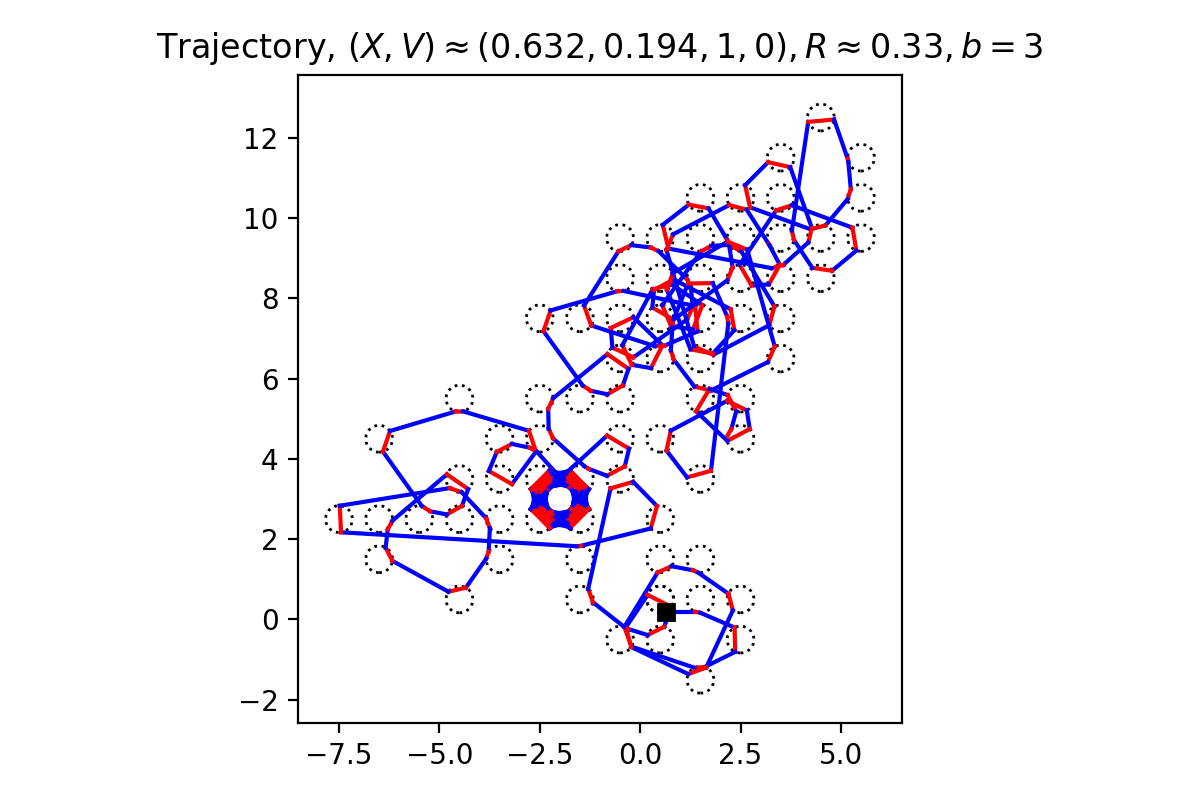
\includegraphics[width=\textwidth, trim={0 0cm 0 0cm}, clip]{sensitive_trajectory.png}
\caption{An example trajectory illustrating various types of motion.}
\label{fig:sensitive_trajectory}
\end{figure}
So far, we see that the motion is not trivial, and warrants study. What is not yet evident from \cref{fig:sensitive_trajectory} is the influence of the parameters $R$ and $b$ on the general behavior of the system. This is what we aim to better understand by the end of the paper. 


We outline how we study this system. We focus on varying $b$, and identify three modes. For some $b_1,b_2\in\mathbb R$ with $0<b_1\ll1<b_2$ \hl{we can also just suggest some values, given our observations},
\begin{enumerate}
\item If $0<b<b_1$, the field strength is low. We can use KAM theory to make sense of quasi-periodicity at these strengths. We find two approaches using KAM.
\item If $b_1<b<b_2$, the field has moderate strength and there is quasi-periodicity of varying complexity. We study this mode, and the next using symbolic dynamics and the Lempel-Ziv complexity measure.
\item If $b_2<b$, the field is strong, and though periodic solutions can be found, we cannot find stable ones.
\end{enumerate}



%\begin{table}[!ht]
%\centering
%\renewcommand\arraystretch{2}
%\begin{tabular}{>{\raggedright}p{0.2\linewidth}
%				>{\raggedright}p{0.2\linewidth}
%				>{\raggedright}p{0.2\linewidth}
%				>{\raggedright\arraybackslash}p{0.2\linewidth}
%                }
%\toprule
% & $b<b_1$ & $b_1<b<b_2$ & $b_2<b$ \\
%\midrule
%Uniform perturbation in a disk 
%  & \multirow{2}*{Usual } 
%  & test cases (difficult in general)
%  & Perturbation of Sinai Billiards (maybe) \\
%Arbitrary perturbations
%  & 
%  & use paper by Donnay-Liverani
%  & Hard?\\
%\bottomrule
%\end{tabular}
%\caption{What it is that we want to do}
%\label{tab:outline}
%\end{table}




